\chapter{VIATRA-CEP}
\label{chap:viatra_cep}
VIATRA-CEP\citep{CEP}\citep{davidi} is the novel Complex Event Processing Framework of the open source VIATRA Project.
In this chapter I overview the tool and the underlying technologies and approaches.

\section{Live model integration}
VIATRA-CEP is built on the top of a live model, in the following novel way:
the user can define graph patterns on the model with VIATRA-Query, and the framework
automatically generates events on every appearance and/or disappearance of these patterns.
The generated events can be used in event patterns, allowing the users to express complex
temporal statements of these patterns. A simplified outline of this architecture is shown in~\cref{fig:viatracep:oldinputs}

%\begin{figure}[h]
%	\centering
%	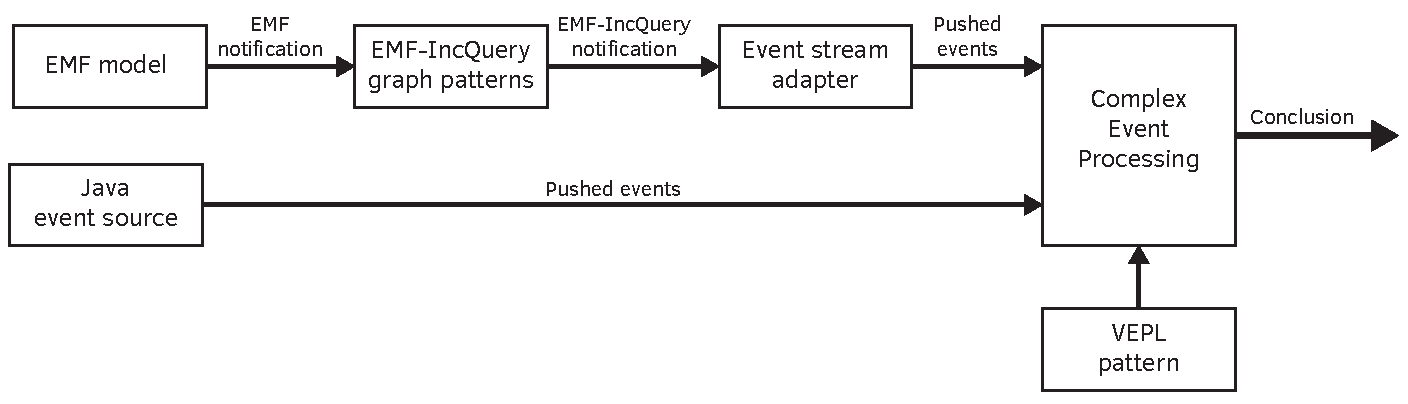
\includegraphics[width=0.9\linewidth]{figures/chapter_3/oldinput}
%	\caption{A brief outline of the live model integration in VIATRA-CEP \redraw}
%	\label{fig:viatracep:oldinputs}
%\end{figure}


\begin{figure}[h]
\noindent
\makebox[\textwidth]{
	\centering
	\begin{tikzpicture}[
	node distance=1cm and 2cm,
	edge/.style={thick, ->}
	]
	\small{
	\node[rect, minimum height=30mm] (cep) {Complex\\Event\\Processing};
	\node[rect, left=of cep, yshift=9mm, xshift=10mm] (es) {Event stream\\adapter};
	\node[rect, left=of es] (vp) {VIATRA-Query\\graph patterns};
	\node[rect, left=of vp, xshift=4mm] (emf) {EMF Model};
	\node[rect, below=of emf] (jes) {Java\\Event Source};
	\node[rect, below=of cep] (vql) {VEPL pattern};
	\node[right=of cep, xshift=-3.5mm] (fakeNode){};
	}
	\footnotesize{
		\draw[edge](emf) -- (vp) node[midway, above, align=center]{EMF\\notification};
		\draw[edge](vp) -- (es) node[midway, above, align=center]{VIATRA-Query\\notification};
		\draw[edge](es) -- (es-|cep.west) node[midway, above, align=center]{Pushed\\Events};
		\draw[edge](jes) -- (jes-|cep.west) node[midway, above, align=center]{Pushed Events};
		\draw[edge](vql) -- (cep);
		\draw[edge](cep) -- (fakeNode) node[midway, above, align=center]{Conclusions};	
	}
	\end{tikzpicture}
}
	\caption{A brief outline of the live model integration in VIATRA-CEP}
	\label{fig:viatracep:oldinputs}
\end{figure}


\section{Event Pattern Language}
VIATRA-CEP uses a language called VIATRA Event Pattern Language (VEPL for short).
This language has intuitive syntax and the event patterns can be defined in
a very high level. 

\paragraph{Operators and semantics}
VEPL basic operators are shown in~\cref{tab:cep:veplop}.
There are additional operators, which can be considered syntactic sugars, shown in~\cref{tab:cep:veplsugar},
but these operators can be expressed with the basic operators as shown in~\cref{tab:cep:veplsugartobasic}, according to \citep{CEP}.

The semantics of the operators ``OR'' and ``AND'' are the following:
\begin{itemize}
	\item operator ``OR'' has a ``committed or'' semantic. This means if that one operand of the ``OR'' is not an atomic event, and that part starts a partial match, the other part of the ``OR'' is ignored while this part is active. \\
	E.g. if the pattern is $(A \rightarrow B)$ OR $C$,
	then trace $A,C$ will not match the pattern.\footnote{Meanwhile VEPL patterns are similar to patterns in regular expressions, they have different semantics. In case of a regular expression, pattern $(AB)|C$ , and the $A\,C$ trace would not cause a match. But since VEPL is used in the field of complex event processing, where an arbitrary prefix for all patterns is set by default, the equivalent of $(A \rightarrow B)$ OR $C$ is $\Sigma^\ast (AB)|C$}
	\item ``AND'' is a binary operator, e.g.~$A$ AND $B$ AND $C$ is equivalent to $(A$ AND $B)$ AND $C$,
	and it will not accept the trace $A\,C\,B$
\end{itemize}

\begin{table}
	\caption{Basic operators}		
	\label{tab:cep:veplop}
	\begin{tabularx}{\textwidth}{llX}
		\toprule
		Operator name             & Denotation                & Meaning                                                                                                                                                                       \\ \midrule
		followed by               & $p_1$ $\rightarrow$ $p_2$ & Both patterns have to appear in the specified order.                                                                                                                          \\
		or                        & $p_1$ OR $p_2$            & One of the patterns has to appear.                                                                                                                                            \\
		``infinite'' multiplicity & $p\{{\ast}\}$             & The pattern can appear 0 to infinite times.                                                                                                                                   \\
		within timewindow         & $p[t]$                    & Once the first element of the complex pattern $p$ is observed (i.e. the patterns ``starts to build up''), the rest of the pattern has to be observed within $t$ milliseconds. \\ \bottomrule
	\end{tabularx}
\end{table}

\begin{table}
	\caption{Syntactic sugars}		
	\label{tab:cep:veplsugar}
	\begin{tabularx}{\textwidth}{llX}
		\toprule
		Operator name                  & Denotation      & Meaning                                                                                                               \\ \midrule
		and                            & $p_1$ AND $p_2$ & Both of the patterns has to appear, but the order does not matter.                                                    \\
		negation                       & NOT $p$         & On atomic pattern: event instance with the given type must not occur. On complex pattern: the pattern must not match. \\
		multiplicity                   & $p\{n\}$        & The pattern has to appear $n$ times, where n is a positive integer.                                                   \\
		``at least once'' multiplicity & $p\{+\}$        & The pattern has to appear at least once.                                                                              \\ \bottomrule
	\end{tabularx}
\end{table}

\begin{table}
	\caption{Syntactic sugars mapped to basic operators}		
	\label{tab:cep:veplsugartobasic}
	\begin{tabularx}{\textwidth}{llX}
		\toprule
		Operator name                  & Denotation      & Equivalent                                                                                            \\ \midrule
		and                            & $p_1$ AND $p_2$ & ($(p_1 \rightarrow p_2)$ OR $(p_2 \rightarrow p_1)$).                                                 \\
		negation                       & NOT $p$         & $\Sigma \setminus p$, where $\Sigma$ is the set of all the possible events.  \\
		multiplicity                   & $p$\{n\}        & $p \rightarrow p \rightarrow \dots p$, n times.                                                       \\
		``at least once'' multiplicity & $p$\{+\}        & $p \rightarrow p\{\ast\}$                                                                             \\ \bottomrule
	\end{tabularx}
\end{table}

\needspace{5cm}
\section{Contexts}

To define properties of execution of the pattern matching, the user can set which event context will be used for the execution.
These event contexts set the properties execution as of noise-reduction, and the maximal amount of partial matches at the same time.

\subsection{Matching and partial matches}
When a pattern is not matched yet, but the current trace is a possible prefix of the pattern, the trace will cause a partial match.
For example, if the pattern is $A \rightarrow B \rightarrow C$, and the trace is $A\;B$ then the pattern matcher only waits for an event $C$.
The event context defines the maximal amount of these partial matches.
For example, if there are multiple matches allowed at the same time, and the pattern is $A \rightarrow B$, the trace $A\;A\;B\;B$ will cause two matches, one at the reception of the first event of type $B$, and one after the reception of the second event of type $B$. 
If only one partial match would be used at the same time, the occurrence  first event of type $B$ would cause a match, but the second occurrence  would not.


\subsection{Noise and noise-reduction}
In most cases, where a Complex Event Processor is used, there are multiple event sources, with vast amount of event types.
Even in these cases, there are many pattern, which does not use all of these event types.
In VIATRA-CEP, the noise is defined as following: An incoming event, which will not increase the size of the currently non-contradictory postfix of the trace.
For example, if the pattern is $A \rightarrow B \rightarrow C$, and the previous trace is $A\;B$, an event $B$ is considered noise. Note that in this example, an event $A$ would not be noise, as it will either start a new partial match, if it is allowed, or restart the matching depending on the chosen context.

\subsection{Overview of the event contexts}

\begin{table}
	\caption{Event Contexts in VIATRA-CEP}		
	\label{tab:cep:contexts}
	\begin{tabularx}{\textwidth}{lcc}
		\toprule
		Context          & Noise-reduction & Partial matches at the same time \\ \midrule
		Strict Immediate &       $-$       &              Single              \\
		Immediate        &       $-$       &             Multiple             \\
		Chronicle        &  $\checkmark$   &             Multiple             \\ \bottomrule
	\end{tabularx}
\end{table}

All three different event contexts introduced in \citep{davidi} are shown in~\cref{tab:cep:contexts}.
These contexts can be defined separately for each event pattern, and they will define the execution semantics of the generated automata. 
An example of these contexts are shown on \cref{tab:cep:contextexample}. In this example the first three rows represent an example of the noise-reduction property, as the Chronicle Context ignores the events in the trace, which are not in the current pattern.
The last three rows represent an example of the multiple partial matches, as the Immediate and the Chronicle Event Contexts have two matches, while the Strict Immediate has only one.
The accepted parts of the traces are under- and overlined from their start to their end.



\begin{table}
	\caption{Examples of the Event Contexts in VIATRA-CEP}		
	\label{tab:cep:contextexample}
	\centering
	\begin{tabular}{@{}clcc@{}}
		\toprule
		  VEPL pattern    & Context          &                             Trace                             &      Accepted       \\ \midrule
		$A \rightarrow B$ & Strict Immediate &                           $A\,C\,B$                           &         $-$         \\[1ex]
		                  & Immediate        &                           $A\,C\,B$                           &         $-$         \\[1ex]
		                  & Chronicle        &                     $\underline{A\,C\,B}$                     &    $\checkmark$     \\[4ex]
		                  & Strict Immediate &                   $A\,\underline{A\,B}\,B$                    &    $\checkmark$     \\[1ex]
		                  & Immediate        & $\mathrlap{\overline{\phantom{AAB}}} A\, \underline{A\,B\,B}$ & $2\times\checkmark$ \\[1ex]
		                  & Chronicle        & $\mathrlap{\overline{\phantom{AAB}}} A\, \underline{A\,B\,B}$ & $2\times\checkmark$ \\[1ex] \bottomrule
	\end{tabular}
\end{table}



\section{Overview of the architecture}
In this section a short overview of the inside of the VIATRA-CEP is given.

The user first optionally defines the graph patterns on an EMF model, or simply defines atomic events.
Using these two, the user builds up complex event patterns, and sets the context for each event pattern. The event patterns are compiled to an automaton
whose execution semantics is defined by the context, as shown on \cref{fig:viatracep:oldcep}. 
Note that the overall semantics is defined by both the automaton generated from the event pattern, and the context.
If the goal is to create an extensible framework, one of the possible approaches is to use a general intermediate language. In this case additional languages only require a mapping to the intermediate language.
A well defined formal intermediate representation supports the formal verification of the CEP specification, and the semantics is desirable to be defined exclusively by the automaton.



\begin{figure}[h]
	\centering
	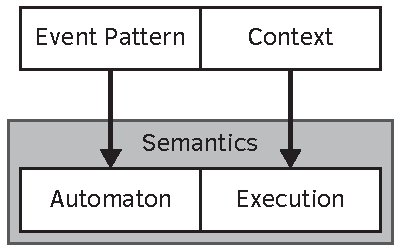
\includegraphics[width=0.4\linewidth]{figures/chapter_3/oldcep}
	\caption{The architectural overview of the VIATRA-CEP}
	\label{fig:viatracep:oldcep}
\end{figure}

\section{Prefiltering functionalities}
In the new (0.13) version of the VIATRA-CEP the traits and the check expression has been introduced to help the user automatize some of the prefiltering functions.

These functionalities are be described here, however these are not in the scope of this thesis, as their implementation is not strictly related to the complex event processing.

\paragraph{Traits}
Traits provide abstraction mechanism to Atomic event patterns. Currently, it supports abstraction of event parameters. For example if the user want to handle all events with coordinateX and coordinateY fields the user can create an abstraction with traits as shown on \cref{fig:viatracep:trait}.


\begin{lstlisting}[caption={Example of the traits in VIATRA-CEP},label={fig:viatracep:trait}]
	trait position {
		coordinateX : double = 0.0, //definition with default value
		coordinateY : double
	}
\end{lstlisting}


\paragraph{Check expressions in atomic events}

Check expressions are helpful to filter the incoming events without unnecessary code-noise in the patterns. For example if the user wishes to get only the events with positive coordinates a check expression can be applied as shown on \cref{fig:viatracep:check}.

\begin{lstlisting}[caption={Example of the Check expression in VIATRA-CEP},label={fig:viatracep:check}]
	atomicEvent object with position {
		check {
			coordinateX > 0 && coordinateY > 0
		}
	}
\end{lstlisting}



\section{Intermediate modeling layer}
Our proposal is to use an intermediate language between the event pattern language and the automata representation, and to use this intermediate language as a common representation of the high level specification, as shown on \cref{fig:viatracep:newcep}. In addition, the long term goal is to support formal analysis of the defined properties. 


\begin{figure}[h]
	\centering
	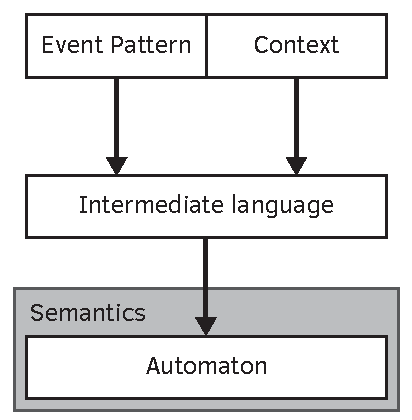
\includegraphics[width=0.4\linewidth]{figures/chapter_3/newcep}
	\caption{The architectural overview of our proposed architecture}
	\label{fig:viatracep:newcep}
\end{figure}


Using an intermediate language increases the extensibility of the framework, as additional pattern languages can be added later, by implementing a compiler from the high level language to the intermediate language, as shown on \cref{fig:viatracep:newinputs}.
The intermediate language would allow the user to combine patterns defined in multiple languages, as multiple automata could run and their simultaneous runs could be analyzed in a formal way.

\begin{figure}[h]
	\noindent
	\makebox[\textwidth]{
		\centering
		\begin{tikzpicture}[
		node distance=1cm and 2cm,
		edge/.style={thick, ->}
		]
		\small{
			\node[rect, minimum height=30mm] (cep) {Complex\\Event\\Processing};
			\node[rect, left=of cep, yshift=9mm, xshift=10mm] (es) {Event stream\\adapter};
			\node[rect, left=of es] (vp) {VIATRA-Query\\graph patterns};
			\node[rect, left=of vp, xshift=4mm] (emf) {EMF Model};
			\node[rect, below=of emf] (jes) {Java\\Event Source};
			\node[rect, below=0cm and 0cm of cep, text width = 19.55mm, inner xsep = 0mm] (il) {Intermediate\\language\\layer};
			\node[rect, below=of il] (vql) {VEPL pattern};
			\node[rect, left=of vql] (additional) {Additional\\languages};
			\node[right=of cep, xshift=-3.5mm] (fakeNode){};
		}
		\footnotesize{
			\draw[edge](emf) -- (vp) node[midway, above, align=center]{EMF\\notification};
			\draw[edge](vp) -- (es) node[midway, above, align=center]{VIATRA-Query\\notification};
			\draw[edge](es) -- (es-|cep.west) node[midway, above, align=center]{Pushed\\Events};
			\draw[edge](jes) -- (jes-|cep.west) node[midway, above, align=center]{Pushed Events};
			\draw[edge](vql) -- (il);
			\draw[edge] (additional.north) |- (il.west);
			\draw[edge](cep) -- (fakeNode) node[midway, above, align=center]{Conclusions};
		} 
		\end{tikzpicture}
	}
	\caption{A brief outline of the live model integration in VIATRA-CEP, with the intermediate language}
	\label{fig:viatracep:newinputs}
\end{figure}
